\documentclass[a4paper]{article}
\usepackage{float}
\usepackage[spanish,es-tabla]{babel}
\usepackage[T1]{fontenc}
\usepackage[spanish]{babel}
\usepackage{graphicx} 
\usepackage[utf8]{inputenc}
\usepackage{amsmath}
\usepackage{longtable} 
\usepackage{amsmath}
\usepackage{graphicx}
\usepackage[colorinlistoftodos]{todonotes}
\usepackage[letterpaper,top=2.5cm,bottom=2.5cm,left=2cm,right=2cm,marginparwidth=2.5cm]{geometry}
\renewcommand{\baselinestretch}{1.25}


\title{Informe Física 8}
\author{Danny Córdova, Edwin Dávila}
\date{21 de Abril del 2023}

\begin{document}

\maketitle

\section{Introducción}

En la presente práctica se estudia el equilibrio mecánico. Dicho equilibrio está compuesto por dos partes: equilibrio traslacional y equilibrio rotacional. El equilibrio traslacional es la ausencia de cambio en la posición del centro de masa de un objeto y se define como: $\sum \Vec{F}_i=0$ (el sumatorio de todas las fuerzas que actúan sobre el cuerpo es igual a 0). Por otro lado, el equilibrio rotacional es la ausencia de rotación sobre un eje de rotación fijo y se define como: $\sum \Vec{\tau}_i=0$ (el sumatorio de todos los torques que actúan sobre el cuerpo es igual a 0). El objetivo de esta práctica es usar el equilibrio mecánico para hacer predicciones teóricas, en este caso, la tensión de las dos cuerdas y contrastar esta información con los valores medidos experimentalmente en la práctica.


\section{Metodología experimental}

Las unidades usadas en este experimento son las del SI. Las incertidumbres de los instrumentos de medida son:

\begin{table}[H]
    \centering
    \begin{tabular}{|c|c|}
    \hline
        Balanza digital & $\pm1 g$ \\ \hline
        Regla  & $\pm 1 mm$ \\ \hline
        Graduador  & $\pm 1^\circ$ \\ \hline
        Dinamómetro & $\pm 20 g$ \\ \hline
    \end{tabular}
    \caption{Incertidumbre de los instrumentos de medida}
    \label{Incertidumbre de los instrumentos de medida}
\end{table}

El experimento se compuso de 2 partes, a continuación se muestra el esquema de ambas partes.

\begin{figure}[H]
    \centering
    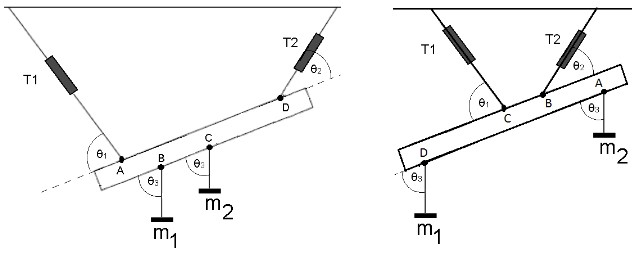
\includegraphics{Esquema exp 8.jpg}
    \caption{Esquema del experimento}
    \label{Esquema}
\end{figure}


Las medidas que se tienen como constantes son: 
\begin{table}[H]
\centering
\begin{tabular}{|c|c|}
    \hline
        Distancia $\overline{AB}$ & $9.1 \pm 1 mm$ \\ \hline
        Distancia $\overline{AC}$ & $20.0 \pm 1 mm$ \\ \hline
        Distancia $\overline{AD}$ & $35.1 \pm 1 mm$ \\ \hline
        Peso de la regla & $716 \pm 1 g$ \\ \hline
        
\end{tabular}
 \caption{Medidas de distancias de la regla}
\end{table}

Las variables directas que se miden en este experimento son:
\begin{enumerate}
  \item Ángulos marcados por cada graduador ($^\circ$).
  \item Tensiones experimentales a través de los dinamómetros ($T_{exp}$).
\end{enumerate}

Las variables indirectas que se calculan a partir de la información obtenida son:
\begin{enumerate}
  \item Tensiones teóricas ($T_{teo}$).
\end{enumerate}

Las fórmulas usadas en este experimento son:

\begin{equation}
    \sum \Vec{F}_i=0
\end{equation}
donde $F_i$ son las fuerzas que actúan sobre un sólido. Esta es la fórmula del equilibrio traslacional.

\begin{equation}
    \sum \Vec{\tau}_i=0
\end{equation}
donde $\tau_i$ son los torques que actúan sobre un sólido. Esta es la fórmula del equilibrio rotacional.

\begin{equation}
    \Vec{\tau}=\Vec{r} \times \Vec{F}
\end{equation}
donde $\tau$ es el torque, F la fuerza, r la posición donde se aplica la fuerza y $\times$ representa el producto cruz. 

\begin{equation}
    P=mg
\end{equation}
donde P es el peso de un objeto, m su masa y g la aceleración de la gravedad.

\begin{equation}
    T_2(1)=\frac{sin(\theta_3)(P x_P+m_2 g x_C +m_1 g x_B)}{sin(\theta_2)(\overline{AD})}
\end{equation}
donde $T_2(1)$ es la tensión 2 mostrada en el esquema del experimento (lado izquierdo).

\begin{equation}
    T_1(1)=\frac{sin(\theta_3)(P+m_1 g+m_2 g)-T sin(\theta_2))}{sin(\theta_2)}
\end{equation}
donde $T_1(1)$ es la tensión 1 mostrada en el esquema del experimento (lado izquierdo) y T es la tensión 2 calculada con (5).

\begin{equation}
    T_1(2)=\frac{sin(\theta_3)(m_1g(\overline{AD}-\overline{AB})+P(\overline{AC}-\overline{AB})-m_2g \overline{AB})}{sin(\theta_1)(\overline{AC}-\overline{AB})}
\end{equation}
donde $T_1(2)$ es la tensión 1 mostrada en el esquema del experimento (lado derecho).

\begin{equation}
    T_2(2)=\frac{sin(\theta_3)(m_2g\overline{AC}-m_1g(\overline{AD}-\overline{AC}))}{sin(\theta_2)(\overline{AC}-\overline{AB})}
\end{equation}
donde $T_2(2)$ es la tensión 2 mostrada en el esquema del experimento (lado derecho).

\begin{equation}
    e=\frac{|T_{teo}-T_{exp}|}{T_{teo}} \times 100\%
\end{equation}
donde $e$ es el error en la medida, $T_{teo}$ la tensión teórica y $T_{exp}$ la tensión experimental.

\section{Resultado y observaciones}

Para el primer caso se tiene su diagrama de cuerpo libre:
\begin{figure} [H]
    \centering
    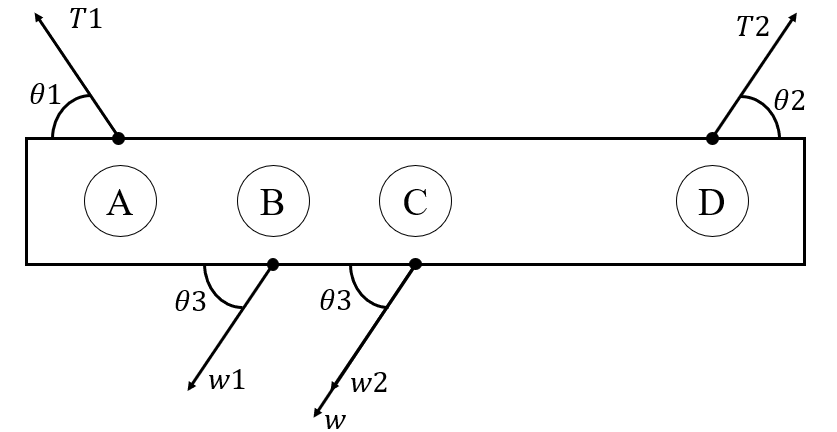
\includegraphics[width=0.6 \textwidth]{Diagrama de cuerpo libre 1.png}
    \caption{Diagrama de cuerpo libre 1}
    \end{figure}

Para este caso se considerará la fórmula (5) y (6) obteniendo de esta manera las tensiones teóricas:

\begin{table}[H]
\centering
\begin{tabular}{l|l|l|l|l|l|l|l|l|l|l|l|l|l|}
\cline{2-14}
                         & 0,05  & 0,1   & 0,15  & 0,2   & 0,25  & 0,3   & 0,35  & 0,4   & 0,45  & 0,5   & 0,55  & 0,6   & 0,65  \\ \hline
\multicolumn{1}{|l|}{$T_{1 exp}$} & 4,091 & 4,457 & 4,821 & 5,185 & 5,529 & 5,885 & 6,248 & 6,617 & 6,980 & 7,334 & 7,705 & 8,068 & 8,430 \\ \hline
\multicolumn{1}{|l|}{$T_{2 exp}$} & 3,879 & 4,006 & 4,130 & 4,255 & 4,395 & 4,527 & 4,653 & 4,772 & 4,898 & 5,031 & 5,149 & 5,275 & 5,400 \\ \hline
\end{tabular}
\caption{Tensiones experimentales 1}
\end{table}

Calculamos el error usando la fórmula (9) y en base a los datos de la tabla ubicada en anexos:

\begin{table}[H]
\centering
\begin{tabular}{l|l|l|l|l|l|l|l|l|l|l|l|l|l|}
\cline{2-14}
                         & 0,05  & 0,1   & 0,15  & 0,2   & 0,25  & 0,3   & 0,35 & 0,4   & 0,45  & 0,5  & 0,55  & 0,6   & 0,65 \\ \hline
\multicolumn{1}{|l|}{$e_{T1}$} & 14,00 & 16,67 & 14,85 & 5,75  & 8,08  & 7,01  & 6,14 & 8,43  & 10,38 & 9,39 & 8,67  & 5,51  & 4,94 \\ \hline
\multicolumn{1}{|l|}{$e_{T2}$} & 10,85 & 14,67 & 13,58 & 14,85 & 11,20 & 12,27 & 9,23 & 10,60 & 7,76  & 8,79 & 10,09 & 11,17 & 8,58 \\ \hline
\end{tabular}
\caption{Errores de tensiones 1}
\end{table}

Obteniendo así como error promedio de $T_1=9,22\%$ y $T_2=11.05\%$

\

\

\


Ahora repetimos el mismo proceso con el segundo caso, su diagrama de cuerpo libre es:
\begin{figure} [H]
    \centering
    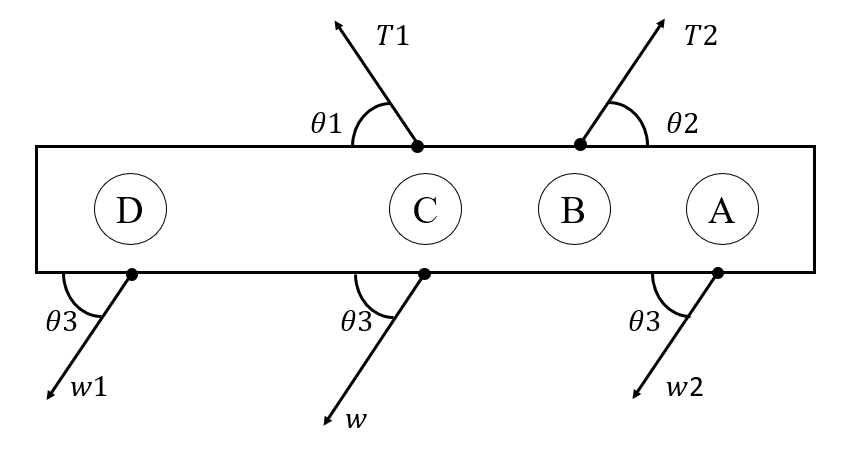
\includegraphics[width=0.6 \textwidth]{Diagrama de cuerpo libre 2.png}
    \caption{Diagrama de cuerpo libre 2}
    \end{figure}

Usando las fórmulas (7) y (8) calculamos las tensiones teóricas: 

\begin{table}[H]
\centering
\begin{tabular}{l|l|l|l|l|l|l|l|l|l|l|l|l|l|}
\cline{2-14}
                         & 0,05  & 0,1   & 0,15  & 0,2   & 0,25  & 0,3   & 0,35  & 0,4   & 0,45  & 0,5   & 0,55  & 0,6   & 0,65   \\ \hline
\multicolumn{1}{|l|}{$T_{1 exp}$} & 0,520 & 2,340 & 2,963 & 3,623 & 4,473 & 5,227 & 5,955 & 6,695 & 7,455 & 8,175 & 8,818 & 9,493 & 10,802 \\ \hline
\multicolumn{1}{|l|}{$T_{2 exp}$} & 7,102 & 6,881 & 6,577 & 6,171 & 5,967 & 5,691 & 5,444 & 5,182 & 4,910 & 4,598 & 4,401 & 4,212 & 3,769  \\ \hline
\end{tabular}
\end{table}

Calculamos el error usando la fórmula (9) y en base a los datos de la tabla ubicada en anexos:

\begin{table}[H]
\centering
\begin{tabular}{l|l|l|l|l|l|l|l|l|l|l|l|l|l|}
\cline{2-14}
                         & 0,05  & 0,1   & 0,15  & 0,2  & 0,25 & 0,3  & 0,35 & 0,4  & 0,45 & 0,5  & 0,55 & 0,6   & 0,65  \\ \hline
\multicolumn{1}{|l|}{$e_{T1}$} & 62,00 & 19,73 & 16,61 & 9,02 & 8,98 & 6,96 & 5,06 & 3,79 & 3,08 & 2,00 & 2,53 & 10,37 & 12,78 \\ \hline
\multicolumn{1}{|l|}{$e_{T2}$} & 6,86  & 0,59  & 1,96  & 1,34 & 1,52 & 2,95 & 0,53 & 1,96 & 0,48 & 2,28 & 7,22 & 7,74  & 1,48  \\ \hline
\end{tabular}
\caption{Errores de tensiones 2}
\end{table}

Finalmente, obtenemos el error promedio de $T_1=12,53\%$ y $T_2=2,84\%$
\section{Conclusiones}

El objetivo principal del experimento se cumplió satisfactoriamente: se pudieron hallar las tensiones de manera teórica para poder compararlas con las tensiones experimentales medidas. Con los datos obtenidos se puede concluir que la condición de equilibrio mecánico sirve para poder hacer predicciones sobre el sistema en estudio. Los errores obtenidos en este experimento son relativamente altos y analizando la metodología del experimento se puede deber principalmente a la incertidumbre del dinamómetro, ya que es una incertidumbre elevada. A pesar de este margen de error, las tensiones experimentales son compatibles y coherentes con las tensiones experimentales.  

\section{Referencias}
\begin{enumerate}
    \item Herrera, N. (2018). \textit{Equilibrio mecánico}.
\end{enumerate}

\section{Anexos}

\begin{table}[H]
\centering
\begin{tabular}{l|l|l|l|l|l|l|l|l|l|l|l|l|l|}
\cline{2-14}
\textbf{}                          & 0,05   & 0,1    & 0,15   & 0,2    & 0,25   & 0,3    & 0,35   & 0,4    & 0,45   & 0,5    & 0,55   & 0,6    & 0,65   \\ \hline
\multicolumn{1}{|l|}{\textbf{$\theta_1$}}   & 87     & 87     & 87     & 88     & 86     & 86     & 86     & 86     & 86     & 86     & 86     & 86     & 87     \\ \hline
\multicolumn{1}{|l|}{\textbf{$\theta_3$}} & 88     & 89     & 89     & 89     & 88     & 88     & 88     & 88     & 88     & 88     & 88     & 88     & 88     \\ \hline
\multicolumn{1}{|l|}{\textbf{$\theta_2$}}   & 84     & 84     & 84     & 84     & 86     & 87     & 87     & 86     & 86     & 87     & 86     & 86     & 86     \\ \hline
\multicolumn{1}{|l|}{\textbf{$T_2$}}  & 4,300 & 4,593 & 4,691 & 4,887 & 4,887 & 5,082 & 5,082 & 5,278 & 5,278 & 5,473 & 5,669 & 5,864 & 5,864 \\ \hline
\multicolumn{1}{|l|}{\textbf{$T_1$}}  & 3,518 & 3,714 & 4,105 & 4,887 & 5,082 & 5,473 & 5,864 & 6,060 & 6,255 & 6,646 & 7,037 & 7,623 & 8,014 \\ \hline
\end{tabular}
\caption{Datos experimentales del esquema 1}
\end{table}

\begin{table}[H]
\centering
\begin{tabular}{l|l|l|l|l|l|l|l|l|l|l|l|l|l|}
\cline{2-14}
\textbf{}                          & 0,05 & 0,1 & 0,15 & 0,2 & 0,25 & 0,3 & 0,35 & 0,4 & 0,45 & 0,5 & 0,55 & 0,6 & 0,65 \\ \hline
\multicolumn{1}{|l|}{\textbf{$\theta_3$}} & 47   & 55  & 65   & 70  & 77   & 82  & 88   & 90  & 93   & 100 & 107  & 112 & 116  \\ \hline
\multicolumn{1}{|l|}{\textbf{$\theta_1$}}   & 127  & 119 & 107  & 96  & 91   & 84  & 77   & 71  & 66   & 61  & 53   & 46  & 43   \\ \hline
\multicolumn{1}{|l|}{\textbf{$\theta_2$}}   & 18   & 23  & 38   & 49  & 56   & 63  & 70   & 76  & 82   & 87  & 95   & 100 & 114  \\ \hline
\multicolumn{1}{|l|}{\textbf{$T_2$}}  & 6,646 & 6,841 & 6,450 & 6,255 & 6,060 & 5,864 & 5,473 & 5,082 & 4,887 & 4,496 & 4,105 & 3,909 & 3,714 \\ \hline
\multicolumn{1}{|l|}{\textbf{$T_1$}}  & 1,368 & 1,955 & 2,541 & 3,323 & 4,105 & 4,887 & 5,669 & 6,450 & 7,232 & 8,014 & 8,601 & 8,601 & 9,578 \\ \hline
\end{tabular}
\caption{Datos experimentales del esquema 2}
\end{table}

\end{document}